\label{sec:control-strategies}

\begin{figure}
    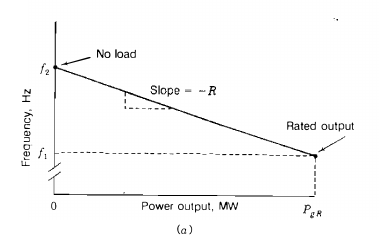
\includegraphics[width=0.8\linewidth]{Images/droop_control.png}
    \captionof{figure}{Linear droop control curve \cite{anderson_power_2003}}
    \label{fig:droop-control}
\end{figure}


The authors of \cite{lin_research_2020} propose the following categorization
of GFM control strategies:
\begin{enumerate}
  \item droop control
  \item virtual synchronous machine (VSM)
  \item virtual oscillating control (VOC)
\end{enumerate}
but they also note that these various strategies share properties in common.
In particular, for all these control strategies, the GFM inverter acts
as a voltage source.

\subsection{Droop Control}
"Droop control" is a term inherited from the classical literature on
SGs, where it presumably refers to the "droop" of the mechanical centrifugal governor
control mechanism. According to \cite{anderson_power_2003},
droop is defined as the relationship
between a generator's change in frequency as the power output varies from no load
to the rated output, per the following equation
\begin{equation}
    R_{pu} = \frac{\delta \omega_{pu}}{P_{rated,pu}}
\end{equation}
where $\delta \omega_{pu}$ is the per-unit change in frequency, $P_{rated,pu}$ is
the per-unit rated power, and $R_{pu}$ is the per-unit droop.

Within the GFM technology, this is the most well-established
control techniques, see \cite{chandorkar_control_1993}. Typically, a linear droop relationship is established
according to
\begin{equation}
  \omega^* = \omega_0 - R (P_* - P)
\end{equation}
where $\omega_*$ is the frequency setpoint of the system, $\omega_0$ is the nominal
frequency, $R$ is the droop characteristic, $P_*$ is the power setpoint, and $P$
is the actual current power (adapted from \cite{chandorkar_control_1993}). The
relative $R$ values throughout the system then determine how power is shared
between devices. Figure (\ref{fig:droop-control})

Recent studies have investigated "nonlinear droop control" which establish a nonlinear
relationship between frequency and real power output. \cite{kenyon_droop-e_2022}
proposes an algorithm called "Droop-e" in which frequency and power are related
by an exponential curve, which "allows greater utilization of available headroom."
In other words, since in any power system the generators must hold some power in reserve
in case of contingencies, a nonlinear relation can allow operation closer to
the system capacity. \cite{kenyon_interactive_2023} also compares various non-linear
droop controls in the mixed GFM/GFL systems. Figure (\ref{fig:droop-control-schematic})
displays a control schematic for a common droop controller.

\begin{figure}
    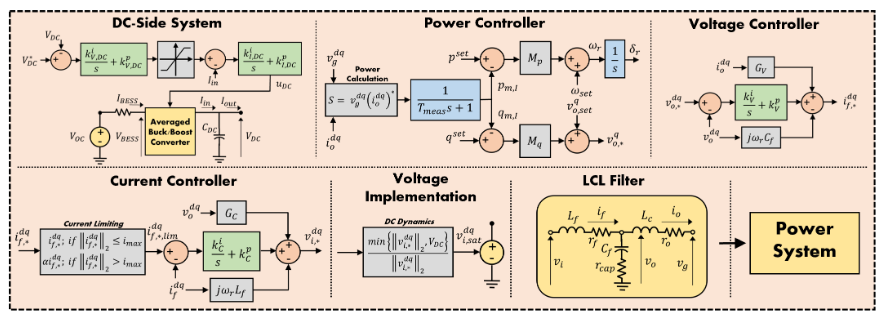
\includegraphics[width=0.8\linewidth]{Images/PE_control_layout.png}
    \captionof{figure}{Droop control schematic \cite{kenyon_interactive_2023}}
    \label{fig:droop-control-schematic}
\end{figure}


\subsection{Virtual Inertia-based Schemes}
Both VSM  strategies aim to emulate SGs by designing controllers
which exhibit similar dynamical properties to an SG. Namely, they 
attempted to emulate the mechanical inertia of SGs, commonly referred
to as virtual inertia (VI).
These methods ensure that the RoCoF after a distrubance remains constrained
within a certain limit. This is important because various components of
power system protection make assumptions on RoCoF, so that changes
in the dynamical properties of underlying generation may invalidate
protection-related assumptions \cite{denholm_inertia_2020}.

\begin{figure}
    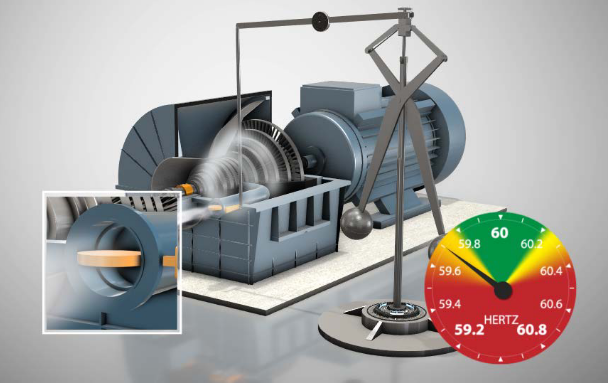
\includegraphics[width=0.8\linewidth]{Images/synchronous_generator.png}
    \captionof{figure}{Inertia and control of synchronous generator \cite{denholm_inertia_2020}}
    \label{fig:synchronous-generator}
\end{figure}

The degree to which it is possible to fully emulate an SG is again driven by 
the physics of the underlying system. For instance, due to the relatively
limited current that PEs, differences in behavior between SG and
VSM-controlled PEs can emerge during fault scenarios \cite{milano_foundations_2018}.
However, VSM control algorithms can provide a good baseline for control algorithm
performance.

It is generally agreed upon that virtual-inertia-based techniques, while serving
as a good starting point are inherently limited in performance since they do not
take capitalize on one of the main advantages of PEs, much faster response times
than SGs \cite{milano_foundations_2018}. \cite{kenyon_interactive_2023} shows
in simulation that although systems with GFMs exhibit faster RoCoF, they also
are able to reduce the maximum deviation from the nominal frequency. 

% \subsection{Optimization-based techniques}

% [TODO: foundations and challenges paper has interesting notes on optimal
% control parameter tuning, etc., read this more thoroughly!]
